\newpage
\section{Eksamensopgave 5 - Kinematik}
\begin{figure}[h!]
    \centering
    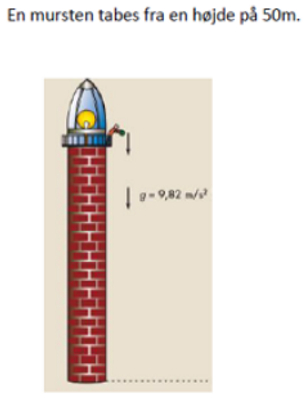
\includegraphics[width=0.3\textwidth]{figures/kinematik.png}
    \caption{Kimenatik opgave}
\end{figure}

\subsection{Beregn murstenens position efter 0,1s}
Først start med at identificer de kendte værdier:
\\\\
Startposition: 50 meter \newline
Start hastighed: 0 m/s (da den falder frit fra hvile position)\newline
Tid: 0,1 sekunder \newline
Tyngdeacceleration: \begin{math}9,82m/s^{2}\end{math}


\subsubsection{Brug den kinematiske formel for position}
Den generelle formel for position ved frit fald er:
\begin{equation*}
    \mathcolorbox{yellow}{s=1/2 \cdot g \cdot t^{2}}
\end{equation*}
s = strækning\newline
g = Tyngdeacceleration\newline
t = tid

\subsubsection{Indsæt værdierne i formlen og udregn}
\begin{equation*}
    \mathcolorbox{yellow}{1/2 \cdot 9,82m/s^{2} \cdot (0,1s)^{2}=0,0491m}
\end{equation*}

Murstenens position efter 0,1s er 49,95m over jorden.

\subsection{Bestem hvor lang tid der går, inden murstenen rammer jorden}

Først identificer vi de kendte værdier som er brugt ovenover

\subsubsection{Brug den kinematiske formel for position}
\begin{equation*}
    \mathcolorbox{yellow}{1/2\cdot g\cdot t^{2}=s}
\end{equation*}
Indsæt værdierne
\begin{equation*}
    \mathcolorbox{yellow}{1/2\cdot9,82m/s^{2}\cdot t^{2}=50m}
\end{equation*}
Dette giver t = 3,191s. Hvilket betyder at der går 3,191s før murstenen rammer jorden.

\subsection{Beregn murstenens hastighed, lige inden den rammer jorden}
For at kunne udregne dett bruger vi formlen nedenunder.
\begin{equation*}
    \mathcolorbox{yellow}{v=a\cdot t}
\end{equation*}
v = velocity\newline
a = acceleration\newline
t = tid
\subsubsection{Indsæt de kendte værdier}
\begin{equation*}
    \mathcolorbox{yellow}{9,82m/s^{2}\cdot 3,191s = 31,34 m/s}
\end{equation*}


\newpage